\subsection{Vehicle measurements}
\label{sec:vehicle}

\subsubsection{Setup}
\label{sec:vehicle-setup}

\subsubsection{Measurement results}
\label{sec:vehicle-meas}

\begin{figure}[htbp]
  \centering
  % GNUPLOT: LaTeX picture with Postscript
\begingroup
  \makeatletter
  \providecommand\color[2][]{%
    \GenericError{(gnuplot) \space\space\space\@spaces}{%
      Package color not loaded in conjunction with
      terminal option `colourtext'%
    }{See the gnuplot documentation for explanation.%
    }{Either use 'blacktext' in gnuplot or load the package
      color.sty in LaTeX.}%
    \renewcommand\color[2][]{}%
  }%
  \providecommand\includegraphics[2][]{%
    \GenericError{(gnuplot) \space\space\space\@spaces}{%
      Package graphicx or graphics not loaded%
    }{See the gnuplot documentation for explanation.%
    }{The gnuplot epslatex terminal needs graphicx.sty or graphics.sty.}%
    \renewcommand\includegraphics[2][]{}%
  }%
  \providecommand\rotatebox[2]{#2}%
  \@ifundefined{ifGPcolor}{%
    \newif\ifGPcolor
    \GPcolorfalse
  }{}%
  \@ifundefined{ifGPblacktext}{%
    \newif\ifGPblacktext
    \GPblacktexttrue
  }{}%
  % define a \g@addto@macro without @ in the name:
  \let\gplgaddtomacro\g@addto@macro
  % define empty templates for all commands taking text:
  \gdef\gplbacktext{}%
  \gdef\gplfronttext{}%
  \makeatother
  \ifGPblacktext
    % no textcolor at all
    \def\colorrgb#1{}%
    \def\colorgray#1{}%
  \else
    % gray or color?
    \ifGPcolor
      \def\colorrgb#1{\color[rgb]{#1}}%
      \def\colorgray#1{\color[gray]{#1}}%
      \expandafter\def\csname LTw\endcsname{\color{white}}%
      \expandafter\def\csname LTb\endcsname{\color{black}}%
      \expandafter\def\csname LTa\endcsname{\color{black}}%
      \expandafter\def\csname LT0\endcsname{\color[rgb]{1,0,0}}%
      \expandafter\def\csname LT1\endcsname{\color[rgb]{0,1,0}}%
      \expandafter\def\csname LT2\endcsname{\color[rgb]{0,0,1}}%
      \expandafter\def\csname LT3\endcsname{\color[rgb]{1,0,1}}%
      \expandafter\def\csname LT4\endcsname{\color[rgb]{0,1,1}}%
      \expandafter\def\csname LT5\endcsname{\color[rgb]{1,1,0}}%
      \expandafter\def\csname LT6\endcsname{\color[rgb]{0,0,0}}%
      \expandafter\def\csname LT7\endcsname{\color[rgb]{1,0.3,0}}%
      \expandafter\def\csname LT8\endcsname{\color[rgb]{0.5,0.5,0.5}}%
    \else
      % gray
      \def\colorrgb#1{\color{black}}%
      \def\colorgray#1{\color[gray]{#1}}%
      \expandafter\def\csname LTw\endcsname{\color{white}}%
      \expandafter\def\csname LTb\endcsname{\color{black}}%
      \expandafter\def\csname LTa\endcsname{\color{black}}%
      \expandafter\def\csname LT0\endcsname{\color{black}}%
      \expandafter\def\csname LT1\endcsname{\color{black}}%
      \expandafter\def\csname LT2\endcsname{\color{black}}%
      \expandafter\def\csname LT3\endcsname{\color{black}}%
      \expandafter\def\csname LT4\endcsname{\color{black}}%
      \expandafter\def\csname LT5\endcsname{\color{black}}%
      \expandafter\def\csname LT6\endcsname{\color{black}}%
      \expandafter\def\csname LT7\endcsname{\color{black}}%
      \expandafter\def\csname LT8\endcsname{\color{black}}%
    \fi
  \fi
    \setlength{\unitlength}{0.0500bp}%
    \ifx\gptboxheight\undefined%
      \newlength{\gptboxheight}%
      \newlength{\gptboxwidth}%
      \newsavebox{\gptboxtext}%
    \fi%
    \setlength{\fboxrule}{0.5pt}%
    \setlength{\fboxsep}{1pt}%
\begin{picture}(7776.00,4320.00)%
    \gplgaddtomacro\gplbacktext{%
      \csname LTb\endcsname%
      \put(682,440){\makebox(0,0)[r]{\strut{}$10$}}%
      \put(682,892){\makebox(0,0)[r]{\strut{}$20$}}%
      \put(682,1344){\makebox(0,0)[r]{\strut{}$30$}}%
      \put(682,1796){\makebox(0,0)[r]{\strut{}$40$}}%
      \put(682,2248){\makebox(0,0)[r]{\strut{}$50$}}%
      \put(682,2699){\makebox(0,0)[r]{\strut{}$60$}}%
      \put(682,3151){\makebox(0,0)[r]{\strut{}$70$}}%
      \put(682,3603){\makebox(0,0)[r]{\strut{}$80$}}%
      \put(682,4055){\makebox(0,0)[r]{\strut{}$90$}}%
      \put(814,220){\makebox(0,0){\strut{}12:10}}%
      \put(1471,220){\makebox(0,0){\strut{}12:20}}%
      \put(2127,220){\makebox(0,0){\strut{}12:30}}%
      \put(2784,220){\makebox(0,0){\strut{}12:40}}%
      \put(3440,220){\makebox(0,0){\strut{}12:50}}%
      \put(4097,220){\makebox(0,0){\strut{}13:00}}%
      \put(4753,220){\makebox(0,0){\strut{}13:10}}%
      \put(5410,220){\makebox(0,0){\strut{}13:20}}%
      \put(6066,220){\makebox(0,0){\strut{}13:30}}%
      \put(6723,220){\makebox(0,0){\strut{}13:40}}%
      \put(7379,220){\makebox(0,0){\strut{}13:50}}%
    }%
    \gplgaddtomacro\gplfronttext{%
      \csname LTb\endcsname%
      \put(176,2247){\rotatebox{-270}{\makebox(0,0){\strut{}\ch{NO2} Concentration [ppb]}}}%
      \csname LTb\endcsname%
      \put(6392,3882){\makebox(0,0)[r]{\strut{}\ch{NO2} ICAD }}%
      \csname LTb\endcsname%
      \put(6392,3662){\makebox(0,0)[r]{\strut{}\ch{NO_x} ICAD}}%
    }%
    \gplbacktext
    \put(0,0){\includegraphics{../images/hd_comparison}}%
    \gplfronttext
  \end{picture}%
\endgroup

  \caption{Comparison of the used CE-DOAS systems. No Ozone was
    entered into either air stream. No systematic effects
    determinable. The difference is
    \SI[separate-uncertainty=true]{-0.37 \pm 0.02}{ppb}.}
  \label{fig:hd-comparison}
\end{figure}
\todo{systematic error of comparison?}
\begin{figure}[htbp]
  \centering
  % GNUPLOT: LaTeX picture with Postscript
\begingroup
  \makeatletter
  \providecommand\color[2][]{%
    \GenericError{(gnuplot) \space\space\space\@spaces}{%
      Package color not loaded in conjunction with
      terminal option `colourtext'%
    }{See the gnuplot documentation for explanation.%
    }{Either use 'blacktext' in gnuplot or load the package
      color.sty in LaTeX.}%
    \renewcommand\color[2][]{}%
  }%
  \providecommand\includegraphics[2][]{%
    \GenericError{(gnuplot) \space\space\space\@spaces}{%
      Package graphicx or graphics not loaded%
    }{See the gnuplot documentation for explanation.%
    }{The gnuplot epslatex terminal needs graphicx.sty or graphics.sty.}%
    \renewcommand\includegraphics[2][]{}%
  }%
  \providecommand\rotatebox[2]{#2}%
  \@ifundefined{ifGPcolor}{%
    \newif\ifGPcolor
    \GPcolorfalse
  }{}%
  \@ifundefined{ifGPblacktext}{%
    \newif\ifGPblacktext
    \GPblacktexttrue
  }{}%
  % define a \g@addto@macro without @ in the name:
  \let\gplgaddtomacro\g@addto@macro
  % define empty templates for all commands taking text:
  \gdef\gplbacktext{}%
  \gdef\gplfronttext{}%
  \makeatother
  \ifGPblacktext
    % no textcolor at all
    \def\colorrgb#1{}%
    \def\colorgray#1{}%
  \else
    % gray or color?
    \ifGPcolor
      \def\colorrgb#1{\color[rgb]{#1}}%
      \def\colorgray#1{\color[gray]{#1}}%
      \expandafter\def\csname LTw\endcsname{\color{white}}%
      \expandafter\def\csname LTb\endcsname{\color{black}}%
      \expandafter\def\csname LTa\endcsname{\color{black}}%
      \expandafter\def\csname LT0\endcsname{\color[rgb]{1,0,0}}%
      \expandafter\def\csname LT1\endcsname{\color[rgb]{0,1,0}}%
      \expandafter\def\csname LT2\endcsname{\color[rgb]{0,0,1}}%
      \expandafter\def\csname LT3\endcsname{\color[rgb]{1,0,1}}%
      \expandafter\def\csname LT4\endcsname{\color[rgb]{0,1,1}}%
      \expandafter\def\csname LT5\endcsname{\color[rgb]{1,1,0}}%
      \expandafter\def\csname LT6\endcsname{\color[rgb]{0,0,0}}%
      \expandafter\def\csname LT7\endcsname{\color[rgb]{1,0.3,0}}%
      \expandafter\def\csname LT8\endcsname{\color[rgb]{0.5,0.5,0.5}}%
    \else
      % gray
      \def\colorrgb#1{\color{black}}%
      \def\colorgray#1{\color[gray]{#1}}%
      \expandafter\def\csname LTw\endcsname{\color{white}}%
      \expandafter\def\csname LTb\endcsname{\color{black}}%
      \expandafter\def\csname LTa\endcsname{\color{black}}%
      \expandafter\def\csname LT0\endcsname{\color{black}}%
      \expandafter\def\csname LT1\endcsname{\color{black}}%
      \expandafter\def\csname LT2\endcsname{\color{black}}%
      \expandafter\def\csname LT3\endcsname{\color{black}}%
      \expandafter\def\csname LT4\endcsname{\color{black}}%
      \expandafter\def\csname LT5\endcsname{\color{black}}%
      \expandafter\def\csname LT6\endcsname{\color{black}}%
      \expandafter\def\csname LT7\endcsname{\color{black}}%
      \expandafter\def\csname LT8\endcsname{\color{black}}%
    \fi
  \fi
    \setlength{\unitlength}{0.0500bp}%
    \ifx\gptboxheight\undefined%
      \newlength{\gptboxheight}%
      \newlength{\gptboxwidth}%
      \newsavebox{\gptboxtext}%
    \fi%
    \setlength{\fboxrule}{0.5pt}%
    \setlength{\fboxsep}{1pt}%
\begin{picture}(8062.00,4320.00)%
    \gplgaddtomacro\gplbacktext{%
      \csname LTb\endcsname%
      \put(814,440){\makebox(0,0)[r]{\strut{}$-10$}}%
      \put(814,842){\makebox(0,0)[r]{\strut{}$0$}}%
      \put(814,1243){\makebox(0,0)[r]{\strut{}$10$}}%
      \put(814,1645){\makebox(0,0)[r]{\strut{}$20$}}%
      \put(814,2047){\makebox(0,0)[r]{\strut{}$30$}}%
      \put(814,2448){\makebox(0,0)[r]{\strut{}$40$}}%
      \put(814,2850){\makebox(0,0)[r]{\strut{}$50$}}%
      \put(814,3252){\makebox(0,0)[r]{\strut{}$60$}}%
      \put(814,3653){\makebox(0,0)[r]{\strut{}$70$}}%
      \put(814,4055){\makebox(0,0)[r]{\strut{}$80$}}%
      \put(946,220){\makebox(0,0){\strut{}14:50}}%
      \put(1693,220){\makebox(0,0){\strut{}15:00}}%
      \put(2439,220){\makebox(0,0){\strut{}15:10}}%
      \put(3186,220){\makebox(0,0){\strut{}15:20}}%
      \put(3932,220){\makebox(0,0){\strut{}15:30}}%
      \put(4679,220){\makebox(0,0){\strut{}15:40}}%
      \put(5425,220){\makebox(0,0){\strut{}15:50}}%
      \put(6172,220){\makebox(0,0){\strut{}16:00}}%
      \put(6918,220){\makebox(0,0){\strut{}16:10}}%
      \put(7665,220){\makebox(0,0){\strut{}16:20}}%
    }%
    \gplgaddtomacro\gplfronttext{%
      \csname LTb\endcsname%
      \put(176,2247){\rotatebox{-270}{\makebox(0,0){\strut{}Concentration [ppb]}}}%
      \csname LTb\endcsname%
      \put(6678,3882){\makebox(0,0)[r]{\strut{}\ch{NO2}}}%
      \csname LTb\endcsname%
      \put(6678,3662){\makebox(0,0)[r]{\strut{}\ch{NO_x}}}%
      \csname LTb\endcsname%
      \put(6678,3442){\makebox(0,0)[r]{\strut{}\ch{NO_{\text{\hphantom{x}}}}}}%
    }%
    \gplbacktext
    \put(0,0){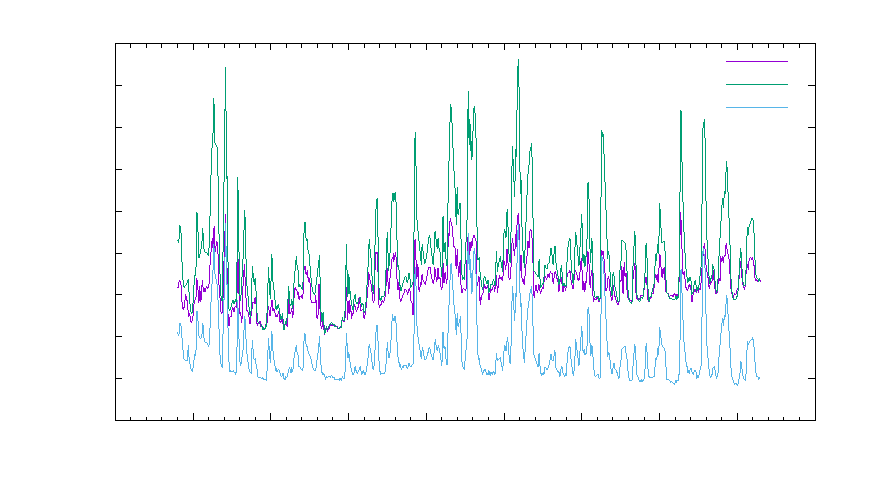
\includegraphics{../images/umba_ts}}%
    \gplfronttext
  \end{picture}%
\endgroup

  \caption{Timeseries of the \ch{NO_x}, \ch{NO2} and the computed
    \ch{NO} concentration next to the Umweltlandesamt air quality
    measurement station in Heidelberg.}
  \label{fig:umba}
\end{figure}

\begin{table}[htbp]
  \centering
  \sisetup{
    table-format=2.1
  }
  \begin{tabular}{c S S}
    \toprule
    {Compound} & \multicolumn{2}{c}{Concentration in \si{ppb}}\\
    & {Station} & {DOAS}\\
    \midrule
    \ch{NO} & 7.4 & 6.5\\
    \ch{NO2} & 19.2 & 21.9\\
    \ch{NOx} & 26.6 & 28.4\\ 
    \bottomrule
  \end{tabular}
  \caption{Comparison between air quality measurement station and
    improved CE-DOAS instrument.}
  \label{tab:umba}
\end{table}

%%% Local Variables:
%%% mode: latex
%%% TeX-master: "../Bachelor"
%%% End:
